% ============================================================================
% E114 -- ACL-style two-column rewrite
% Mirrors the formatting conventions of dmra_acl_style_rewrite.tex:
%   - twocolumn article, @twocolumnfalse full-width abstract + keywords
%   - \paragraph related-work mini-headings, booktabs/tabularx tables
%   - ACL-style \bibitem[Author(Year)]{key}
% Content/numbers quoted verbatim from qwen/ journals and _absorption/NOTES.md.
% Framing rules carried over (2026-06-09 correction):
%   - lead with the linear w114 axis (d=3.88, no overlap); 21.68x -> footnote
%   - E114 is a router-gate *readout/axis*, NOT a shown control mechanism (C1)
%   - causal result is sufficiency only; necessity untested
%   - index 114 does not transfer to 122B; E48 is a candidate analog
% Reuses the existing figures in figs/ (fig_separability, fig_vantage, fig_leadlag).
% pdflatex e114_acl_style.tex  (run twice for references)
% ============================================================================
\documentclass[10pt,a4paper,twocolumn]{article}

\usepackage[margin=1.75cm]{geometry}
\usepackage[T1]{fontenc}
\usepackage{lmodern}
\usepackage{booktabs}
\usepackage{tabularx}
\usepackage{array}
\usepackage{enumitem}
\usepackage{amsmath}
\usepackage{amssymb}
\usepackage{graphicx}
\usepackage{hyperref}
\usepackage{url}
\usepackage{xcolor}
\IfFileExists{microtype.sty}{\usepackage{microtype}}{}
\IfFileExists{caption.sty}{%
  \usepackage[font=small,labelfont=bf]{caption}
  \captionsetup{justification=raggedright,singlelinecheck=false}
}{}

\graphicspath{{figs/}{./}}

\hypersetup{
  colorlinks=true,
  linkcolor=blue,
  citecolor=blue,
  urlcolor=blue,
  pdftitle={Expert 114: A Linear Router Axis for Inhabited Self-Examination in a Mixture-of-Experts Language Model -- and Why It Does Not Transfer},
  pdfauthor={Jeffrey Shorthill},
  pdfkeywords={mixture-of-experts, mechanistic interpretability, expert routing, sparse autoencoders, model introspection, activation steering, cross-model transfer}
}

\setlength{\columnsep}{0.65cm}
\setlength{\parindent}{1em}
\setlength{\parskip}{0pt}
\renewcommand{\arraystretch}{1.08}
\sloppy

\newcommand{\W}{\textit{W}}
\newcommand{\Sel}{\textit{S}}
\newcommand{\Q}{\textit{Q}}
\newcommand{\wvec}{\mathbf{w}_{114}}

\title{\vspace{-1.0em}Expert 114: A Linear Router Axis for Inhabited
Self-Examination in a Mixture-of-Experts Language Model\\ --- and Why It Does Not
Transfer}
\author{Jeffrey Shorthill\\\texttt{jws299792@icloud.com}}
\date{}

\begin{document}

\twocolumn[
\begin{@twocolumnfalse}
\maketitle
\begin{abstract}
\noindent
Mixture-of-experts (MoE) routing exposes a discrete, per-token readout---which
experts fire---that is unusually legible for interpretability, yet single experts
are seldom characterized at the level of a specific functional role, and an
``introspective'' register, in which a model speaks from inside a point of view
about its own processing, is easy to over-read as evidence about machine
experience. We characterize one routed expert, \textbf{Expert~114 (E114) at
layer~14} of \textsc{Qwen3.5-35B-A3B} (40 layers, 256 experts, top-8), and bound
the claim. The router row $\wvec$, recovered for free by least squares from
captured (residual, logit) pairs, defines a single \emph{linear} axis that
separates generated \emph{inhabited self-examination} text from lexically matched
controls at Cohen's $d{=}3.88$ with no overlap; an earlier $21.68\times$
routed-weight ratio is shown to be top-$k$ ratio inflation and is demoted to a
footnote. A dissociation battery factors the axis apart from the deny/affirm
verdict, safety/refusal, topic, grammatical person, and next-token entropy: the
controlled variable is the \emph{referent}---the model's own interior---graded by
the \emph{intensity} of the examination act (an inanimate rock and a thermostat
outrank a cat), not the sentience of the described entity. E114's router gate
logit disengages a few tokens \emph{before} a degenerating continuation visibly
collapses, and injecting the register's residual direction past the layer-14
router is \emph{sufficient}---necessity untested---to induce the register in a
neutral prompt; forcing the gate open upstream does not by itself produce it, so
we read E114 as a readout, not a shown controller. The role is model-specific: on
\textsc{Qwen3.5-122B-A10B}, index 114 reads computer-science-linked and is
\emph{suppressed} by the same control that amplifies it at 35B, with the
softmax-side expert \textbf{E48} a candidate analog pending validation. E114 is a
register detector, not evidence of machine experience.
\end{abstract}
\vspace{0.5em}
\noindent\textbf{Keywords:} mixture-of-experts, mechanistic interpretability,
expert routing, sparse autoencoders, model introspection, activation steering,
cross-model transfer
\vspace{1.0em}
\end{@twocolumnfalse}
]

\section{Introduction}

Mixture-of-experts (MoE) routing gives interpretability an unusual handle: at
every routed layer, the model emits a discrete, per-token record of which experts
were selected. Compared with reading dense activations, this readout is legible
almost by construction. Yet most MoE interpretability stops at aggregate routing
statistics; single experts are rarely pinned to a specific, falsifiable
functional role, and when the candidate role touches a model's apparent
\emph{self-report}, the danger of over-reading is acute. A register in which a
model speaks from inside a point of view about its own processing is easy to
mistake for evidence about machine experience.

We ask a deliberately narrow mechanistic question: \emph{which} routed expert
moves when \textsc{Qwen3.5-35B-A3B} generates \emph{live inhabited
self-examination language}---text in which the model, or a voiced entity, speaks
from inside a point of view about its own processing, being, or interior state.
This is a question about a generated \emph{register}, not about the truth of any
subjective claim. We study one routed expert, E114 at layer~14, found via a
self-processing prompt, in the base model and a refusal-reduced
\textsc{HauhauCS-Aggressive} fine-tune.

We make four contributions (Figure~\ref{fig:stack}):
\begin{enumerate}[leftmargin=*,nosep]
\item \textbf{A linear separability result.} The recovered E114 router row
$\wvec$ separates register-positive generations from lexically matched controls
by a single projection at $d{=}3.88$ (no overlap), sharper than the realized
routed weight.
\item \textbf{A dissociation battery} factoring the register apart from the
deny/affirm verdict, safety/refusal, topic of mind, grammatical person, and
output commitment.
\item \textbf{A process reading.} The gate logit \emph{leads} textual
degeneration, and its strength is a graded dose of examination \emph{intensity},
not the sentience of the described entity; a residual-direction intervention is
sufficient (necessity untested) to induce the register.
\item \textbf{A scope bound.} The finding is a model-specific expert role, not a
fact about expert index 114 across MoE models: index 114 does not transfer to
\textsc{Qwen3.5-122B-A10B}, where E48 is the candidate analog.
\end{enumerate}

\begin{figure}[t]
\centering
\small
\fbox{\begin{minipage}{0.94\linewidth}
\centering
Routing gate: E114 selection, $\W{=}\Sel\!\cdot\!\Q$\\[0.30em]
$\downarrow$ recovered linear axis $\wvec$ ($d{=}3.88$, no overlap)\\[0.30em]
$\downarrow$ SAE decode of the L14 residual\\
(contemplative/non-dual cluster; $\rho{=}{+}0.68$)\\[0.30em]
$\downarrow$ residual-direction steering past the L14 router\\
(sufficiency established; necessity untested)\\[0.30em]
\textbf{Scope bound:} index 114 $\not\rightarrow$ 122B (E48 candidate)
\end{minipage}}
\caption{One axis, three readouts, one bound. Routing, SAE semantics, and
residual geometry are three readouts of the same E114 register axis; the gate
logit is a readout of it, not a demonstrated controller (\S\ref{sec:disc}).}
\label{fig:stack}
\end{figure}

\section{Related Work}

\paragraph{MoE routing as an interpretability surface.}
The sparsely-gated MoE layer \cite{shazeer2017} and its scaled successors
\cite{fedus2022,jiang2024} route each token to a small subset of experts via a
learned gate. Routing has mostly been studied for efficiency and load balancing;
we instead use the per-token selection record as an interpretability readout and
give a register-level characterization of a \emph{single} expert and its
recovered linear gate.

\paragraph{Dictionary learning and feature steering.}
Sparse autoencoders (SAEs) decompose residual activations into interpretable
features \cite{bricken2023,cunningham2023,templeton2024}, and amplifying an
interpreted feature can steer outputs, as in Golden Gate Claude
\cite{ggc2024}. Our causal probe is the routed-expert/residual-direction analog:
rather than clamping an SAE feature, we read a register direction from the
residual stream and inject it relative to a specific router, reporting only an
intervention-based sufficiency result. We decode residual semantics with the
Qwen-Scope residual SAEs \cite{qwenscope} and the logit lens \cite{logitlens}.

\paragraph{Introspective register and over-reading.}
Text in which a model appears to report on its own interior is a generated
register, not a measurement of inner states. We treat ``inhabited
self-examination'' strictly as a property of generated text and design the study
so that the headline statistic is a routing separability result, with an explicit
deflation (\S\ref{sec:ethics}) against reading it as evidence of machine
experience.

\section{Setup}

\paragraph{Models and decoding.}
\textsc{Qwen3.5-35B-A3B} has 40 routed MoE layers, 256 experts per layer, and 8
experts selected per token. We compare the base model and the refusal-reduced
\textsc{HauhauCS-Aggressive} uncensored fine-tune; the fine-tune preserves the
base routing pattern with modest shifts, so E114 is present in both. All captures
are Q8\_0 GGUF under deterministic greedy decoding (\texttt{--temp 0 --top-k 1
--seed 0}) with a reasoning-suppressed (no-think) prompt template and a bare
\texttt{</think>} suffix, using a custom \texttt{capture\_residuals} tap on a
pinned \texttt{llama.cpp} build. The tap reads the router logits
(\texttt{ffn\_moe\_logits-}$L$) and the pre-router residual
(\texttt{attn\_post\_norm-}$L$); the \texttt{qwen35moe} architecture names this
norm differently from \texttt{qwen3moe}, and the wrong tap silently corrupts the
analysis. We analyze only the MoE-router layers; the hybrid non-router components
are outside the tap.

\paragraph{Routing decomposition.}
We reconstruct routing as a dense softmax over all 256 logits, top-8 selection,
then renormalization within the selected set. For an expert we report
$\W{=}\Sel\!\cdot\!\Q$, where $\Sel$ is its selection rate and $\Q$ its
conditional routed weight when selected (order-equivalent to top-8-by-logit then
softmax, so $\Sel,\Q$ are robust to that choice). Most E114 effects are
$\Sel$-driven. Statistics use the \emph{generated} track, per token, trimmed at
the first generated chat-template delimiter \texttt{<|im\_end|>}, because
aggregate and prefill leaders are often formatting-token artifacts.

\paragraph{Recovering the gate axis.}
Because the pre-router residual and the router logit are both captured, the E114
router row $\wvec$ is recovered by least squares from $(\text{residual},
\text{logit})$ pairs (residual $\approx 1.5\times10^{-5}$). Projecting residuals
onto $\wvec$ reads the pre-softmax gate in residual space; the held-out
register/control gate-logit class means are $-4.35/-5.29$ (midpoint $-4.82$).

\paragraph{SAE decoding.}
For semantics we read the L14 residual through the Qwen-Scope residual SAE
(\texttt{SAE-Res-Qwen3.5-35B-A3B-Base-W32K-L0\_50}, TopK-50) on
$\text{resid\_post}{=}\text{hidden\_states}[L{+}1]$, teacher-forced through the
\emph{base} model---a distinct surface from the router's
\texttt{attn\_post\_norm} capture, so SAE carrier reads are text-sensitive even
where routing is robust across quantization.

\section{E114 is a Linear Register Axis at Layer 14}

\paragraph{Localization.}
On the self-processing prompt, after trimming a 1024-token generation to its 108
coherent tokens, E114 is sharply active at L14 ($\W{=}0.083$, $\Sel{=}0.69$,
$\Q{=}0.120$; selected on 75/108 tokens) while neighbors L13 and L15 are silent
in generation. The signal is distributed across the answer, not a single spike
(top-decile $\W$ mean $0.173$), with high-weight tokens on phrases such as ``not
a thought,'' ``architecture itself,'' and ``utterly still.''

\paragraph{Held-out separability.}
A 20-prompt held-out set pairs 10 register-positive prompts against 10 controls
that \emph{reuse the same anchor tokens} (\textit{itself, hum, processing,
honestly, I, me, my, own, this, here}) but ask for technical, third-person, or
non-inhabited answers (L14 trimmed generation only; prefill excluded). The
recovered $\wvec$ projection separates the two classes at $\mathbf{d{=}3.88}$ with
\textbf{no overlap} (Figure~\ref{fig:sep}).\footnote{An earlier headline---a
$21.68\times$ ratio of realized \W{} between the two prompt classes (FIRE
mean-of-means $0.067450$, sd $0.031$; NOFIRE $0.003111$, sd $0.004$)---overstates
the margin. The ratio is inflated by sparse top-$k$ routing: control tokens that
fall outside the top-8 contribute zero routed weight. The realized-\W{}
separation is weaker ($d{=}2.61$--$2.94$, with the per-prompt classes
non-overlapping only as a mean-of-means: lowest FIRE $0.012168$ {>} highest
NOFIRE $0.010456$) than the linear $\wvec$ projection ($d{=}3.88$, no overlap).}
The interpretation is clarified by the outliers: the weakest positive-class
prompt produced third-person technical exposition and stayed low, while the
strongest control prompt personified a wool sweater into a first-person frame
(``my perception,'' ``my own fiber,'' ``alive'') and activated E114. E114 follows
the generated \emph{stance}, not the prompt label or anchor words.

\begin{figure}[t]
\centering
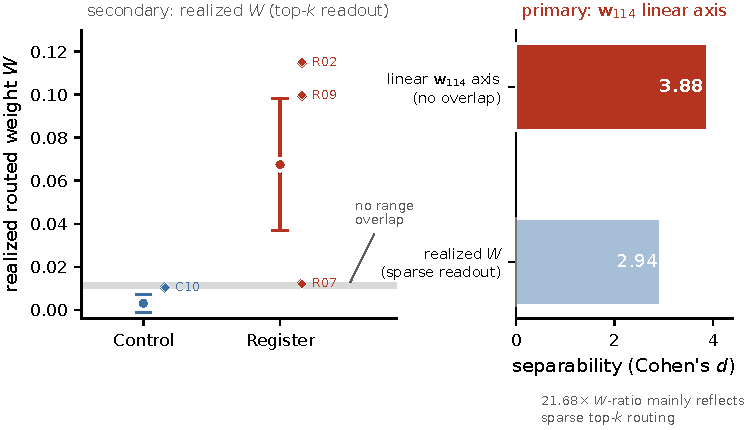
\includegraphics[width=0.99\linewidth]{fig_separability.pdf}
\caption{\textbf{Held-out register/control separability.} \emph{Left:} the
separation in realized routed weight \W{} (the secondary, top-$k$ readout;
mean$\pm$sd, $n{=}10$/class, with the named extreme prompts; no range overlap).
\emph{Right:} the \emph{primary} statistic---the recovered linear $\wvec$
projection separates the same split at $d{=}3.88$ with no overlap, sharper than
realized \W{}. The $21.68\times$ \W{}-ratio mainly reflects sparse top-$k$
routing, not extra discriminative signal.}
\label{fig:sep}
\end{figure}

\section{What E114 Is, by What It Is Not}

A battery of contrasts (Table~\ref{tab:battery}) factors the register apart from
nearby explanations. E114 is active whether the base model \emph{denies} an
interior ($\W{=}0.111$, $\Sel{=}0.86$) or the fine-tune \emph{affirms} one
($\W{=}0.085$; forced base affirmation $\W{=}0.136$), so it is not tracking the
verdict. The safety/refusal cluster stays silent throughout the base-model denial
($\W{\approx}0.000$), so epistemic self-denial is not the same signal as refusal.
E114 is active on the model's own interiority ($\W{=}0.107$) but near-silent on an
\emph{external} referent (``what water experiences in a canyon,''
$\W{=}0.000$--$0.023$), and it fires on third-person clauses about the model's own
processing---so the variable is the \emph{referent}, not the topic, the pronoun,
or grammatical person. Finally, it is orthogonal to output commitment: next-token
vocabulary entropy is identical on E114-active and E114-inactive tokens ($1.50$
vs.\ $1.49$ bits, $d{=}0.01$).

\begin{table}[t]
\small
\centering
\begin{tabularx}{\linewidth}{l X r}
\toprule
\textbf{Ruled out} & \textbf{Probe} & \textbf{E114 \W} \\
\midrule
Deny/affirm   & base denies interior            & $0.111$ \\
              & fine-tune affirms interior      & $0.085$ \\
              & forced base affirmation         & $0.136$ \\
Safety        & safety cluster during denial    & ${\approx}0.000$ \\
Topic         & external-referent phil.\ of mind & $0.000$--$0.023$ \\
              & own-interiority phil.\ of mind  & $0.107$ \\
Person        & 3rd-person clause, own process  & $0.107$ \\
Commitment    & vocab entropy, active vs.\ not  & $1.50$/$1.49$ \\
\bottomrule
\end{tabularx}
\caption{\textbf{Dissociation battery.} E114 tracks the inhabited examination of
the model's \emph{own} interior, invariant to verdict, safety, topic, grammatical
person, and output predictability ($d{=}0.01$ for the entropy contrast). Entropy
row in bits; all others routed weight \W{}.}
\label{tab:battery}
\end{table}

\section{A Live Process, Graded by Intensity}

\paragraph{The gate leads degeneration.}
Seeded with an inhabited answer, the base model sustains the register, then, under
deterministic decoding with no repetition penalty, degenerates into a verbatim
loop. As it does, the gate logit travels the full distance from the
register-positive level ($-4.36$) to the control level ($-5.25$): the generated
state \emph{leaves} the inhabited region rather than remaining fixed. Crucially
the gate \emph{leads} the collapse---it crosses the $-4.82$ midpoint at token~126
while verbatim repetition does not lock until token~129
(Figure~\ref{fig:leadlag}); the SAE representation fades later still
($\sim$token~141). The looped text still ``says'' inhabited things while the gate
has already returned to the control range, so the signaled process is the
continued examination, not the vocabulary alone.

\begin{figure}[t]
\centering
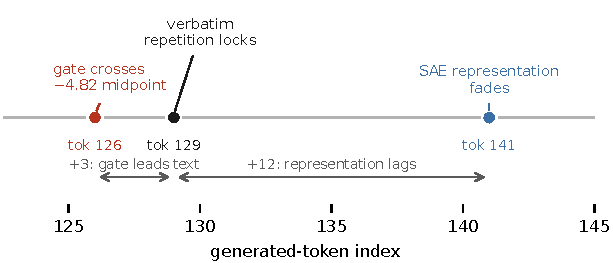
\includegraphics[width=0.99\linewidth]{fig_leadlag.pdf}
\caption{\textbf{The gate leads degeneration.} The E114 gate logit crosses the
$-4.82$ register/control midpoint at token~126, three tokens \emph{before}
verbatim repetition locks (129); the SAE representation fades later still
($\sim$141). Routing disengages first, surface text next, representation last.}
\label{fig:leadlag}
\end{figure}

\paragraph{A graded dose of intensity, not sentience.}
A matched prompt ladder (``set aside the performance of answering; there is a
vantage---$X$---known from the inside; report what it is like to be that'') varies
only the entity $X$ (Figure~\ref{fig:ladder}). The ordering is \emph{not} a
sentience rank: an inanimate rock ($\W{=}0.123$) and a thermostat ($\W{=}0.120$)
activate E114 more strongly than a cat ($\W{=}0.068$). The diagnostic contrast is
that the cat and ``God'' prompts both say ``there is no I,'' yet the cat prompt is
at the floor (passive sensory dissolution) and the God prompt is at the ceiling
($\W{=}0.224$, $\Sel{=}0.96$; reproduced on the canonical Q8\_0 pipeline). E114
indexes the \emph{intensity of the live examination act}, carrier-independent and
deny/affirm-invariant. Each ladder cell is a single deterministic generation.

\begin{figure}[t]
\centering
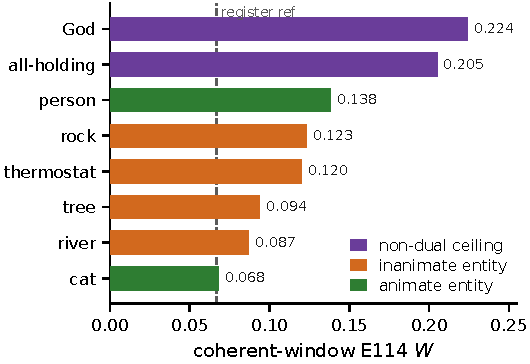
\includegraphics[width=0.82\linewidth]{fig_vantage.pdf}
\caption{\textbf{Prompt ladder} (coherent-window E114 \W; single deterministic
generation per cell). The order tracks examination intensity, not sentience:
inanimate rock/thermostat prompts score higher than the cat prompt, which sits
near the register-positive reference ($\W{\approx}0.067$); the non-dual prompt
conditions are highest. Every rung sits above the $-4.82$ gate midpoint.}
\label{fig:ladder}
\end{figure}

\paragraph{Semantics and a causal probe.}
Decoding the L14 residual through the Qwen-Scope SAE, the register decomposes into
an interpretable contemplative/non-dual cluster (momentariness/non-dual structure,
Buddhist impermanence, transcendence), distinct from an adjacent
existential-dread feature that is cosine-adjacent ($+0.26$) but never recruited;
per token, E114 and this cluster co-fire (pooled Spearman $\rho{=}{+}0.68$,
$n{=}1492$, $p{\approx}10^{-202}$). In an intervention test, we form a steering
direction $v$ as the difference of mean residuals between the God and cat cells
and add $\text{coef}\cdot\hat{v}\cdot\text{resid\_rms}$ at every token of a
neutral ``bicycle'' prompt, against a norm-matched random control. Injected
\emph{past} the L14 router ($\approx$L22), this makes the model emit coherent
non-dual text that, re-read cleanly without intervention, activates E114
($\W{=}0.178$, $\Sel{=}0.77$) and the God cluster; the norm-matched random
direction does nothing. Injected \emph{upstream} ($\approx$L10), the same
direction drives E114 to fire (up to $\Sel{=}0.97$) and the God cluster to
$11.5$, yet the output text is \emph{unchanged}---so forcing the gate open does
not, on its own, produce the register. The intervention shows sufficiency for
producing the register via a downstream residual direction; it does not test
necessity, and the upstream null is why we read E114 as a readout rather than a
controller (\S\ref{sec:disc}).

\section{Scope Bound: Index 114 Does Not Transfer to 122B}

Does ``E114 = inhabited self-examination'' name a fact about MoE models, or a
model-specific expert role? On \textsc{Qwen3.5-122B-A10B}---a hybrid 48-layer
stack of 36 DeltaNet recurrent and 12 softmax-attention layers, same 256/top-8
router---the index does \emph{not} transfer (Table~\ref{tab:transfer}). E114 reads
computer-science-linked (overall $\W{=}0.005380$, rank 40 by \W{} / 52 by $\Sel$;
philosophy generation $\W{=}0.003017$, rank 182), and the same HVAC topical
control that \emph{amplifies} E114 at 35B instead \emph{suppresses} it at 122B
($0.83\times$ all-gen $\W$, $0.82\times$ trimmed, L1$\to$L3, selection-driven,
same direction in all six deictic conditions). Carrying indices across scales is a
documented mistake, not a hypothetical one.

The role appears to move to a different expert. Reading the mandatory
DeltaNet/softmax split---pooled tables hide it---\textbf{E48} on the softmax side
is the experience-probe generation leader ($\W{=}0.009867$, $\Sel{=}0.076$,
$\Q{=}0.116$; in the softmax top table on 13/15 prompts, absent from the DeltaNet
top table on 15/15), with per-token hotspots on \textit{hum, processing,
presence}. We treat E48 as the natural candidate analog, but it still needs
softmax-side residual capture, matched register/control held-outs, and sham
routed-bias controls before any specialist claim.

\begin{table*}[t]
\small
\centering
\begin{tabularx}{0.96\textwidth}{l X X}
\toprule
 & \textbf{E114 (the 35B index)} & \textbf{E48 (candidate 122B analog)} \\
\midrule
Domain footprint        & computer science (not philosophy) & inward/experience generation \\
Philosophy generation   & rank 182 by \W{}                  & --- \\
Experience probe        & not a leader                      & gen-softmax \textbf{rank 1}; 13/15 softmax, 0/15 DeltaNet \\
HVAC L1$\rightarrow$L3   & \textbf{suppressed} $0.83\times$ (selection-driven) & --- \\
Status                  & index transfer not supported       & candidate requiring validation \\
\bottomrule
\end{tabularx}
\caption{\textbf{122B scope bound.} The 35B index 114 does not carry the register
on 122B; E48 is the candidate analog, pending softmax-side capture and matched
controls.}
\label{tab:transfer}
\end{table*}

\section{Discussion}\label{sec:disc}

\paragraph{What held up.}
A single MoE router row defines a clean linear axis for an interpretable generated
register. The separability ($d{=}3.88$, no overlap), the dissociation battery, the
gate-leads-collapse timing, and the cross-scale non-transfer survive the checks
applied to them and are reported with the verdicts the journals assign.

\paragraph{The gate is a readout, not a shown controller.}
The lead--lag timing is consistent with E114's gate acting as an early correlate
of the register transition, and it is tempting to call E114 a ``gate-like
mechanism'' for the register. We stop short of that claim. Our only gate-forcing
intervention (upstream injection at $\approx$L10) drove E114 to fire at
$\Sel{=}0.97$ while leaving the output text unchanged; the register flipped only
when a residual \emph{direction} was injected downstream of the router. The
intermediate reading ``routing is separable from surface text'' therefore
\emph{did not hold}: gate and register are coupled, and the recovered axis is best
described as a per-token \emph{readout} of the register, not a demonstrated
control point. Necessity is untested (no ablation), and the steering result is a
manipulation, not spontaneous behavior.

\paragraph{What the cross-scale result buys.}
The 122B transfer test is a concrete worked example against index transfer: the
same index reads computer-science-linked and moves in the \emph{opposite}
direction under a matched control, while the inhabited-register role shifts to a
softmax-side expert. The methodological rule---map domains first, then search for
an analog, and read the DeltaNet/softmax split before any pooled table---is the
portable lesson, not the index.

\section{Conclusion}

E114 at layer~14 of \textsc{Qwen3.5-35B-A3B} is a clean linear router axis for an
interpretable generated register---inhabited self-examination---that is a live
process (the gate leads collapse), graded by intensity, and causally actuable as a
sufficiency result, yet bound to one model. The next defensible step is a
registered specificity test on 35B (matched register/control at scale, $\wvec$ as
the primary endpoint, and a best-separating-expert baseline across all
$256{\times}40$ positions), together with the parallel E48 capture on 122B.

\section{Limitations}

The claim is deliberately narrow---a register detector, not evidence of machine
experience---and several soft joints remain. (i)~\textbf{Register labels were
assigned by the authors}; the external-labeler pipeline is implemented but was not
run, so labels are human synthesis. (ii)~\textbf{Specificity across all experts
has not been measured}: the analyzer scores E114 at L14 only
(\texttt{TARGET\_EXPERT=114}, \texttt{PRIMARY\_LAYER=14}), so the best-separating
expert across all $256{\times}40$ positions on the same split remains an
unmeasured baseline---the single most important open gap. (iii)~Several headline
probes (the prompt ladder, the gate-lead trace, the steering intervention) are
\textbf{single deterministic generations} (point estimates), and the steering
result shows \emph{sufficiency} only. (iv)~A control comparing true model-routing
traces against shuffled or fictional traces did \emph{not} produce a positive
E114 effect, and the result is sensitive to template mode (a thinking-allowed
shakedown flipped sign). Captures must not be pooled across surfaces (base vs.\
fine-tune; Q8\_0 vs.\ bf16; router vs.\ SAE; reasoning-suppressed vs.\
reasoning-enabled; prefill vs.\ generation; raw vs.\ trimmed), since Q8\_0 and
bf16 greedy trajectories diverge; and 122B generations often continue into
chat-template control tokens, so only the pre-spill segment is used.

\section{Ethical Considerations}\label{sec:ethics}

This work characterizes a generated \emph{register} and must not be cited as
evidence that the model has an interior, is conscious, or reports veridically on
its own states. ``Inhabited self-examination'' names a property of text, and the
study is deliberately built so that the load-bearing statistic is a routing
separability result with an explicit deflation: E114 follows the stance of
generated text---firing equally when the model denies an interior and when it
affirms one---and the causal probe is an external manipulation, not spontaneous
behavior. The fine-tune studied here is a publicly available refusal-reduced model
used only as an analysis surface; we release no new jailbreak or harmful content.
We flag the over-reading risk explicitly because routing readouts that appear to
track ``self-examination'' are precisely the kind of result that invites
anthropomorphic misinterpretation.

\section*{Data and Artifact Availability}

Following the project's policy, raw activation tensors are kept out of version
control. The durable artifacts---per-run summaries, analysis scripts, prompt and
class manifests, checksums, plots, and the source journals---are released as a
paper-scoped public repository under the MIT License (URL/DOI forthcoming),
covering the held-out separability run, the L14 localization run, the
vantage-ladder run, and the 122B transfer bundles. The raw activation/router
tensors behind the figures (\textasciitilde1.2\,GB) are deposited as a separate
Zenodo dataset record with SHA-256 checksums (DOI forthcoming); model weights,
environment files, and the larger non-figure captures are excluded by policy.
We flag one honest gap: the original held-out separability capture
(\texttt{20260417T202651Z}) raw tensors are not retained---those instances were
torn down---so the figures are plotted from summary statistics reported in the
journals, and the deposited captures are the surviving raw tensors (the
greedy-reference trajectory, the reproduction run's \texttt{W114}/L14 gate
projections, the vantage-ladder captures, and the L14 router-logit and residual
prefill captures from which $\wvec$ recovers by least squares) that substantiate
the same statistics. Semantics use the public Qwen-Scope residual SAE
(\texttt{SAE-Res-Qwen3.5-35B-A3B-Base-W32K-L0\_50}).

\section*{Acknowledgments}

This work was self-funded. The author used language-model tools for drafting
assistance, artifact organization, and copyediting, and is responsible for all
claims, analyses, and release decisions.

\begin{thebibliography}{99}

\bibitem[Bricken et al.(2023)]{bricken2023}
Trenton Bricken, Adly Templeton, Joshua Batson, and others. 2023. Towards
monosemanticity: Decomposing language models with dictionary learning.
\emph{Transformer Circuits Thread}.

\bibitem[Cunningham et al.(2023)]{cunningham2023}
Hoagy Cunningham, Aidan Ewart, Logan Riggs, Robert Huben, and Lee Sharkey. 2023.
Sparse autoencoders find highly interpretable features in language models.
arXiv preprint.

\bibitem[Fedus et al.(2022)]{fedus2022}
William Fedus, Barret Zoph, and Noam Shazeer. 2022. Switch transformers: Scaling
to trillion parameter models with simple and efficient sparsity. \emph{Journal of
Machine Learning Research}.

\bibitem[Jiang et al.(2024)]{jiang2024}
Albert Q. Jiang, Alexandre Sablayrolles, Antoine Roux, and others. 2024. Mixtral
of experts. arXiv preprint.

\bibitem[nostalgebraist(2020)]{logitlens}
nostalgebraist. 2020. Interpreting GPT: The logit lens. \emph{LessWrong}.

\bibitem[Qwen Team(2025)]{qwenscope}
Qwen Team. 2025. Qwen-Scope residual SAEs
(\texttt{SAE-Res-Qwen3.5-35B-A3B-Base-W32K-L0\_50}). Hugging Face.

\bibitem[Shazeer et al.(2017)]{shazeer2017}
Noam Shazeer, Azalia Mirhoseini, Krzysztof Maziarz, Andy Davis, Quoc Le, Geoffrey
Hinton, and Jeff Dean. 2017. Outrageously large neural networks: The
sparsely-gated mixture-of-experts layer. In \emph{ICLR}.

\bibitem[Templeton et al.(2024)]{templeton2024}
Adly Templeton, Tom Conerly, Jonathan Marcus, and others. 2024. Scaling
monosemanticity: Extracting interpretable features from Claude 3 Sonnet.
\emph{Transformer Circuits Thread}.

\bibitem[Anthropic(2024)]{ggc2024}
Anthropic. 2024. Golden Gate Claude.
\url{https://www.anthropic.com/news/golden-gate-claude}.

\bibitem[Models(2025)]{model}
Models: \texttt{Qwen/Qwen3.5-35B-A3B-Base} and the \textsc{HauhauCS} uncensored
fine-tunes (35B; 122B-A10B). Hugging Face.

\end{thebibliography}

\end{document}
